% Q12 -- 4x4 barrel shifter. Same 16-transistor grid, but gates are tied
% DIAGONALLY to just 4 shift-control lines sh0..sh3 (staircase). The label in
% each cell is the shift line that drives it: sh_{(j-i) mod 4}.
\documentclass[border=10pt]{standalone}
\usepackage{tikz}
\usetikzlibrary{arrows.meta}
\begin{document}
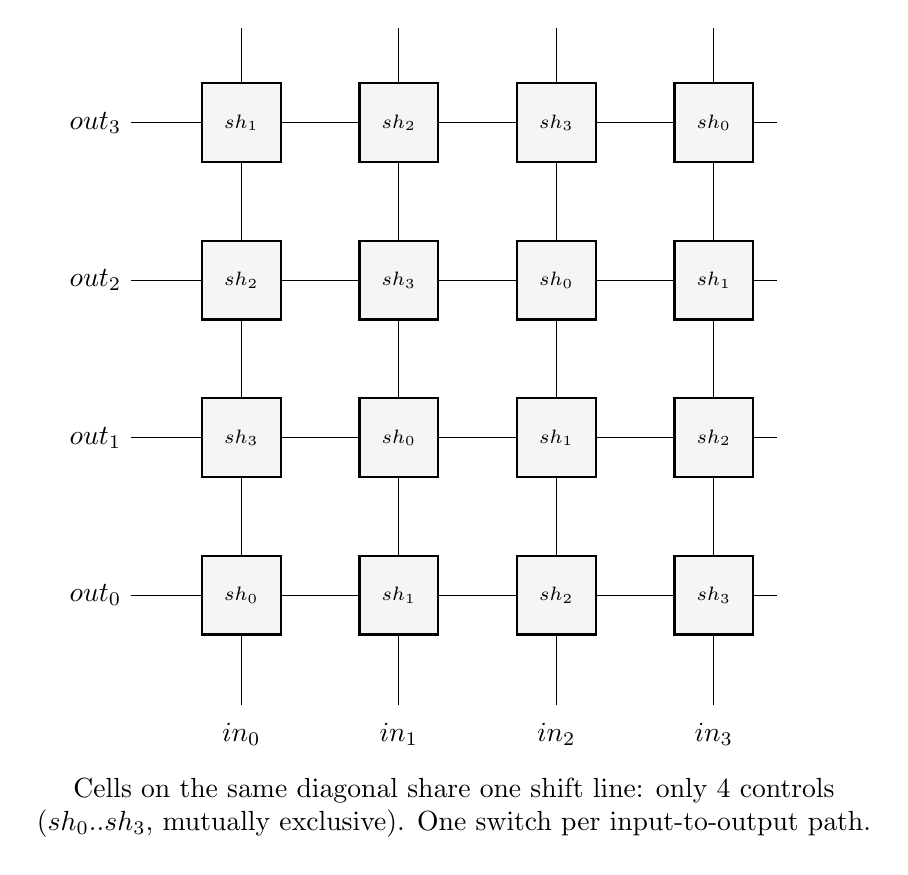
\begin{tikzpicture}[>=Latex, sw/.style={draw, thick, minimum size=1.0cm, fill=black!4}]
\foreach \j in {0,1,2,3}{
  \draw (1.6+2*\j,0.2) -- (1.6+2*\j,8.8);
  \node[below] at (1.6+2*\j,0.1) {$in_{\j}$};
}
\foreach \i/\y in {3/7.6,2/5.6,1/3.6,0/1.6}{
  \draw (0.2,\y) -- (8.4,\y);
  \node[left] at (0.2,\y) {$out_{\i}$};
}
\foreach \i/\y in {3/7.6,2/5.6,1/3.6,0/1.6}{
  \foreach \j in {0,1,2,3}{
    \pgfmathtruncatemacro{\k}{mod(\j-\i+4,4)}
    \node[sw] at (1.6+2*\j,\y) {\scriptsize $sh_{\k}$};
  }
}
\node[align=center] at (4.3,-1.1)
 {Cells on the same diagonal share one shift line: only 4 controls\\
  ($sh_0$..$sh_3$, mutually exclusive). One switch per input-to-output path.};
\end{tikzpicture}
\end{document}
